\documentclass[12pt]{article}
\usepackage[utf8]{inputenc}
\usepackage{amsmath, amssymb}
\usepackage{algpseudocode}
\usepackage{graphicx}
\usepackage{hyperref}
\usepackage{amsthm}
\usepackage{xcolor}

\setlength\parindent{0pt}
\newcommand\note[1]{\textcolor{red}{\textbf{#1}}}


\title{Parallel Odd-Even Sort}
\author{Lorenzo Beretta (\texttt{lorenzo2beretta@gmail.com})}
\date{6th July 2020}

\begin{document}
\maketitle

\section{Introduction}
In this report we implemented two parallel versions of the Odd-Even
Sort (OES) algorithm. The algorithm is pretty simple and works as follows:
we proceed repeating identical iterations, each of which consists of two
scans over the vector to be sorted; the first scan compare elements in
even positions with their successors and, if out of order, swaps
them, the same happens for odd-positioned elements in the subsequent
scan. For the rest of this report we assume to sort a vector $v$ of
length $n$; it can be proven
(\href{https://en.wikipedia.org/wiki/Odd\%E2\%80\%93even_sort}{Wikipedia
Odd-Even Sort})
that $n$ such identical iterations are sufficient to sort the vector,
leading to a sequential complexity of $\mathcal{O}(n^2)$, sub-optimal
with respect to the well known $\mathcal{O}(n\log(n))$ alternatives.
However this algorithm presents a strong data independence (i.e. its data
flow graph is moderately interconnected), therefore we can aim at
achieving interesting speedups with a parallel version.

\section{Design Choices}
The most trivial parallel implementation of OES exploits the data
parallelism that is inherent to the inner for loops; we can simply run
two parallel for (one for the even phase and one for the odd one)
inside a sequential loop. An OMP implementation of this pattern is
provided (\texttt{openmp.cpp}), however the experimental results
showed that the parallel version introduce so much overhead that it is not even compensated by
the speedup, so that the parallel version is slower than the
sequential one. We implemented the exact same pattern implementing the
barrier and the parallel for
by myself (\texttt{pthread-barrier.cpp}) and again it yielded awful
performances. Therefore we decided to get rid of the barriers, it
required some effort and we needed to add some additional structures
and to disrupt the iterative form in which the sequential version has
been describing. In the next section we describe two different
patterns implemented respectively using native C++ threads and the
Fastflow library.


\section{Pthread Version}
We refer to the file \texttt{pthread-async.cpp} that is widely
commented, consider reading the source code for a thorough explanation of
implementation details. The basic idea here is that, given $nw$ workers, we can
partition our vector $v$ in $nw$ chunks, so that each worker only
deals with a single chunk. This is more or less what happens in our
pthread implementation of the ``barrier pattern'' (i.e. the one employing
a parallel for). In that case we synchronized our workers so that they
waited each other once they finished a single pass over their chunk, but now we want to
avoid the overhead arising from that. If we suppose that threads act
really independently many problems open up: first we need to deal with
data races (that we previously neglected, since the odd-even structure
coupled with barriers
prevented any data race); second we need to provide some stopping
condition (since the theorem mentioned in the introduction and stating
that $n$ outer-loop iterations are enough holds only if the outer loop
is sequential).

Now we explain how we managed to solve those problems, implementing a
version of the algorithm in which each worker perform the OES
iterations on its chunks until a global stopping condition is met.

\subsection{Data Races}
Consider the vector $v$ divided in chunks so that the $i$-th chunk is
$v[st[i]] \dots v[en[i]]$ where $st$ and $en$ are suitable vectors of
indices denoting chunk boundaries. Our algorithm swaps elements with
their successors, hence the only elements of $v$ for which a data race
occurs are $v[en[i]] = v[st[i + 1]]$ for some $i = 1 \dots nw$. We can use a vector
of mutexes (one for each of those values) without incurring in a
substantial overhead, in fact each pass over a chunk will only need
two locks and unlocks: one for the left side and one for the
right side boundary. In the next subsection more structure will be
introduced that will need some synchronization mechanism to avoid data
races, we exploited the fact that those structures are often accessed
simultaneously to boundary elements of $v$ and employed the same
mutexes. The only detail worth mention regards deadlocks, to prevent
the deadlocks we adopted the ``topological sort rule'': given the
natural numeration of mutexes associated to elements $v[st[i]]$, we
only nested mutexes so that the inner one is associated with the lower
number.

\subsection{Stopping Condition}
Every thread only operates on its portion of the data performing a
loop indefinitely, how can we set up a stopping condition? We define a
boolean vector $sorted[1\dots nw]$ such that the following invariant
holds: $sort[i]$ is true if and only if both an even and an odd pass
  over the $i$-th chunk have been completed and the following
  properties hold:
\begin{itemize}
\item no transposition was performed during the last
  odd-even phase by the $i$-th worker
  \item no transposition concerning elements at the boundary with the
    $i$-th chunk was performed by $(i + 1)$-th nor $(i -
    1)$-th workers since the beginning of the last odd-even phase of
    the $i$-th thread
\end{itemize}
These two conditions together ensure that the $i$-th chunk is sorted,
therefore if $sorted[i] == true$ for each $i = 1 \dots nw$ then the
algorithm should terminate. This is handled through a global counter
$cnt$ counting how many entries of $sorted$ are set to $true$; clearly
$cnt$ data races are prevented using a mutex. Finally some care should
be taken to set and unset the $sorted$ entries, in fact we need to both
remember its state before the beginning of the current odd-even
iteration and to annotate whether a neighbouring thread swapped any
boundary element, this is achieved using another vector $meanwhile$
that is true if and only if a boundary transposition happened since
the beginning of the current odd-even iteration.

\section{FastFlow Version}
In the Fastflow implementation we implemented a different pattern. We
used a master-worker pattern, namely we declared an emitter node and
$nw$ worker nodes, each equipped with a feedback channel feeding the
emitter. A first approach would be to synchronize all the workers so
that the emitter handles the outer loop of the sequential OES and
workers perform the inner loop exploiting the data parallelism. As
noted above, this kind of barrier introduce a huge overhead, therefore
we opted for a slightly more clever implementation: the key
observation is that the interaction of chunks is only local, therefore
to ensure sequential equivalence it is sufficient to guarantee that
adjacent chunks have a ``lag'' of at most one odd or even iteration.
More formally, we
consider odd and even iterations as distinct and define the vector
$npass[1\dots nw]$ counting how many odd (or even) passes have been
performed over the $i$-th chunk; then we start the $j$-th pass over
the $i$-th chunk only if $npass[i + 1] \geq j$ and $npass[i - 1] \geq j$.
We need lower bound of the number of passes in order to ensure
correctness, hence in a first version of this pattern the emitter
updated the number of passes (performing
\texttt{++npass[i]}) when a worker signaled that has finished its work
using the feedback loop. This was further improved, in fact it is
sufficient to immediately perform the boundary transpositions
(directly performed by the emitter) in order to increment $npass$
without affecting correctness; in fact the external view of the chunk
depends only on its boundary elements. In this way we achieved some
decent speedups that we will see in the experiments section.

In the design of the FF version we checked that each thread was mapped
to a different core of the Xeon Phi machine we run all our experiments
on, this ensured that, using less workers than physical cores, the
SPSC non-blocking FIFO was more efficient (although more power
consuming) than the blocking version. Moreover we confronted different
scheduling policies and found out that the default one (loose round
robin) was the most efficient one.

\section{Experiments}
All the experiments have been performed on the Xeon Phi machine
\footnote{Architecture: x86\_64, CPUs: 256, Cores 64, 1.30GHz, 64-bit.} 
whose access has been provided during the course. Our primary goal in
the experiment was to evaluate the speedup and scalability achieved by
our two implementations. For this reason we implemented a sequential
version (\texttt{sequential.cpp}) and compared the performances.

We used vectors of random integers generated from a console-provided
seed, so that we could guarantee the fairness of the experiments
(reduce the random noise introduced by differently shuffled
vectors). Although the code is written for a vector of integers, it is
very easy to generalize it to a generic type for which a total order
operator \texttt{<} is defined. It is apparent that if we choose more
costly comparison function speedup  will get better
(by Gustafson's law), therefore in this sense we explored a ``worst case
scenario''.

All the experiments were performed over a sample size of 10 trials
(with different, but fixed, starting seeds) and
a random vector of length $10^5$ integers. Here we report plots
showing the average throughput and the ideal one (i.e. the one
obtained from the sequential multiplying by the number of workers).
We present two plots showing the throughput achieved by our parallel
implementations by
(\texttt{ff-farm.cpp} and \texttt{pthread-async.cpp}) against the number of
workers $nw$.

\begin{figure}[H]
  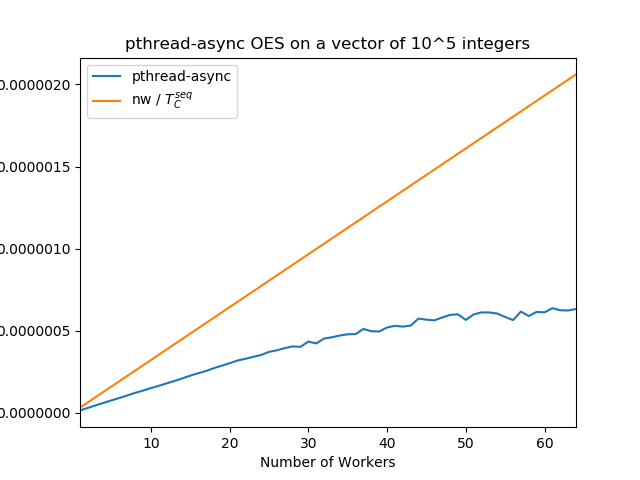
\includegraphics{pthread-async_speedup.png}
  \caption{This figure shows the throughput of pthread-async (it would
  lie on the yellow line if the maximum speedup was achieved)}
\end{figure}
\begin{figure}[H]
  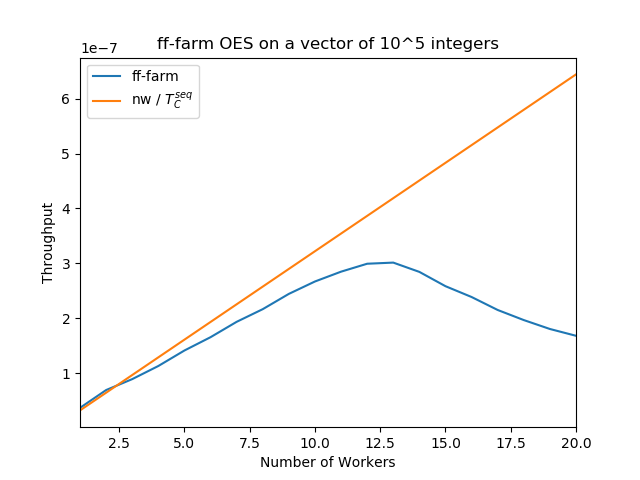
\includegraphics{ff-farm_speedup.png}
  \caption{This figure shows the throughput of pthread-async (it would
  lie on the yellow line if the maximum speedup was achieved)}
\end{figure}

Overall we achieved pretty good speedups, although it is clear that
there is a difference in ``responsiveness'' to the number of workers between the two.
We can notice that the pthread version scale worse for low values of
$nw$ but is more steady for $nw > 10$, on the contrary the Fastflow
version is better while the number of worker is small and get much
worse when we add more workers.

  


\bibliographystyle{acm}  
\bibliography{biblio}
\end{document}

%%% Local Variables:
%%% mode: latex
%%% TeX-master: t
%%% End:
